\chapter{Set Theory: Building the Mathematical Universe}

\section{Why Sets?}

\begin{intuition}
We've learned logic---how to reason correctly. Now we need \textit{objects} to reason about.

What are the basic building blocks of mathematics? Numbers? Functions? Shapes?

The answer might surprise you: \textbf{everything is a set}.

Numbers are sets. Functions are sets. Even the operations we perform (+, ×, etc.) are sets. Set theory is the ``assembly language'' of mathematics---everything reduces to it.
\end{intuition}

\subsection{What Is a Set? (Naively)}

Let's start informally before we encounter problems.

\begin{definition}[Naive Definition---FLAWED!]
A \textbf{set} is a collection of distinct objects, called its \textbf{elements} or \textbf{members}.
\end{definition}

\begin{example}[Familiar Sets]
\begin{itemize}
    \item $\{1, 2, 3\}$ = the set containing the numbers 1, 2, and 3
    \item $\{a, b, c\}$ = the set of the first three letters
    \item $\{\text{red}, \text{blue}, \text{green}\}$ = a set of colors
    \item $\mathbb{N} = \{0, 1, 2, 3, \ldots\}$ = the natural numbers
    \item $\emptyset = \{\}$ = the empty set (no elements)
\end{itemize}
\end{example}

\subsection{Basic Notation}

We write $x \in A$ to mean ``$x$ is an element of set $A$.''

We write $x \notin A$ to mean ``$x$ is not an element of set $A$.''

\begin{center}
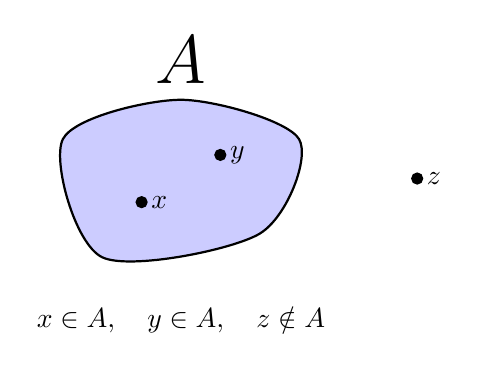
\begin{tikzpicture}
    % Draw a set as a blob
    \draw[thick, fill=blue!20] plot[smooth cycle] coordinates {(0,0) (2,0.3) (2.5,1.5) (1,2) (-0.5,1.5)};
    \node at (1,2.5) {\Huge $A$};
    
    % Elements inside
    \filldraw (0.5,0.7) circle (2pt) node[right] {$x$};
    \filldraw (1.5,1.3) circle (2pt) node[right] {$y$};
    
    % Element outside
    \filldraw (4,1) circle (2pt) node[right] {$z$};
    
    \node[below] at (1,-0.5) {$x \in A,\quad y \in A,\quad z \notin A$};
\end{tikzpicture}
\end{center}

\subsection{Key Properties of Sets}

From our naive definition, sets have these properties:

\begin{enumerate}
    \item \textbf{Order doesn't matter}: $\{1, 2, 3\} = \{3, 2, 1\} = \{2, 1, 3\}$
    
    \item \textbf{Repetition doesn't matter}: $\{1, 2, 2, 3, 3, 3\} = \{1, 2, 3\}$
    
    \item \textbf{Elements are distinct}: A set either contains an element or it doesn't---no multiples
    
    \item \textbf{Membership is definite}: For any object $x$ and set $A$, either $x \in A$ or $x \notin A$ (no ambiguity)
\end{enumerate}

\begin{example}[Order and Repetition]
\begin{center}
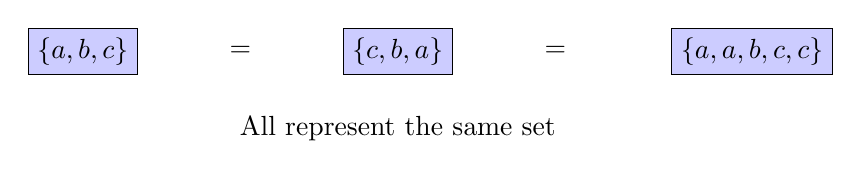
\begin{tikzpicture}
    \node[rectangle, draw, fill=blue!20] at (0,0) {$\{a, b, c\}$};
    \node at (2,0) {$=$};
    \node[rectangle, draw, fill=blue!20] at (4,0) {$\{c, b, a\}$};
    \node at (6,0) {$=$};
    \node[rectangle, draw, fill=blue!20] at (8.5,0) {$\{a, a, b, c, c\}$};
    \node[below] at (4,-0.7) {All represent the same set};
\end{tikzpicture}
\end{center}
\end{example}

\section{The Crisis: Russell's Paradox}

Everything seems fine so far. But there's a catastrophic problem with our naive definition!

\begin{historicalnote}
In 1901, Bertrand Russell discovered a devastating paradox that showed naive set theory was \textbf{inconsistent}---it led to contradictions.

This was like discovering a crack in the foundation of a skyscraper. Mathematicians had to tear down and rebuild the foundations of mathematics.
\end{historicalnote}

\subsection{Sets Can Contain Sets}

First, note that sets can contain other sets as elements:

\begin{example}
\begin{itemize}
    \item $\{\{1, 2\}, \{3, 4\}\}$ = a set containing two sets
    \item $\{1, \{2, 3\}\}$ = a set containing a number and a set
    \item $\{\emptyset\}$ = a set containing the empty set (NOT the same as $\emptyset$!)
\end{itemize}
\end{example}

\begin{center}
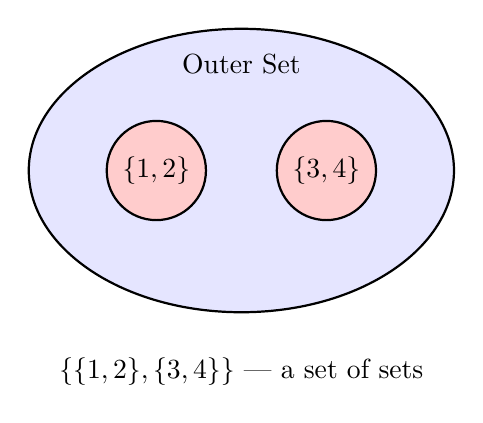
\begin{tikzpicture}[scale=0.9]
    % Outer set
    \draw[thick, fill=blue!10] (0,0) ellipse (3cm and 2cm);
    \node at (0,1.5) {Outer Set};
    
    % Inner sets
    \draw[thick, fill=red!20] (-1.2,0) circle (0.7cm);
    \node at (-1.2,0) {$\{1, 2\}$};
    
    \draw[thick, fill=red!20] (1.2,0) circle (0.7cm);
    \node at (1.2,0) {$\{3, 4\}$};
    
    \node[below] at (0,-2.5) {$\{\{1,2\}, \{3,4\}\}$ --- a set of sets};
\end{tikzpicture}
\end{center}

Question: Can a set contain \textit{itself}?

\subsection{The Paradox}

\begin{theorem}[Russell's Paradox]
Consider the ``set'' $R = \{x \mid x \notin x\}$ (``the set of all sets that don't contain themselves'').

\textbf{Question:} Is $R \in R$?

\begin{itemize}
    \item \textbf{If $R \in R$}: Then $R$ contains itself. But by definition of $R$, it only contains sets that DON'T contain themselves. So $R \notin R$. Contradiction!
    
    \item \textbf{If $R \notin R$}: Then $R$ doesn't contain itself. But that's exactly the criterion for being in $R$! So $R \in R$. Contradiction!
\end{itemize}

Both possibilities lead to contradiction. Therefore, $R$ cannot exist!
\end{theorem}

\begin{center}
\begin{tikzpicture}[node distance=2cm]
    \node[rectangle, draw, fill=yellow!20, text width=2.5cm, align=center] (assume1) {Assume\\$R \in R$};
    \node[rectangle, draw, fill=red!20, text width=3cm, align=center, right=3cm of assume1] (contra1) {Then $R \notin R$\\Contradiction!};
    \draw[->, thick] (assume1) -- (contra1);
    
    \node[rectangle, draw, fill=yellow!20, text width=2.5cm, align=center, below=2.5cm of assume1] (assume2) {Assume\\$R \notin R$};
    \node[rectangle, draw, fill=red!20, text width=3cm, align=center, right=3cm of assume2] (contra2) {Then $R \in R$\\Contradiction!};
    \draw[->, thick] (assume2) -- (contra2);
    
    \node[below=1.5cm of assume2, text width=7cm, align=center] {\textbf{No consistent answer!}\\Naive set theory is broken.};
\end{tikzpicture}
\end{center}

\begin{keyidea}
Russell's Paradox shows that we \textbf{cannot} allow arbitrary collections to be sets. The phrase ``the set of all sets that...'' is too permissive.

We need \textbf{axioms} that carefully restrict which collections are sets, avoiding contradictions.
\end{keyidea}

\begin{remark}[Classes versus Sets]
Russell's Paradox reveals a fundamental distinction that must be made precise:

\begin{itemize}
    \item \textbf{Sets} are the objects of study in ZFC set theory. They can be members of other sets. The axioms of ZFC carefully control which collections form sets.
    
    \item \textbf{Proper Classes} are collections ``too large'' to be sets. For example:
    \begin{itemize}
        \item The collection of all sets (the ``universal class'')
        \item Russell's collection $\{x \mid x \notin x\}$
        \item The collection of all ordinal numbers (defined later)
    \end{itemize}
    
    Classes can be described by formulas but \textbf{cannot be members} of other collections in ZFC.
\end{itemize}

\textbf{Why ZFC Avoids the Paradox:}

In ZFC, we don't have a ``set of all sets.'' When we write $\{x \mid \varphi(x)\}$, this notation only makes sense when restricted by the Axiom of Separation (or Replacement), which forms sets from existing sets, never from ``all objects.''

For instance, the Axiom of Separation allows us to form
\[
\{x \in A \mid x \notin x\}
\]
for any set $A$, but not the unrestricted collection $\{x \mid x \notin x\}$.

\textbf{Alternative Foundation: NBG Set Theory}

Some authors use von Neumann–Bernays–Gödel (NBG) set theory, which explicitly includes both sets and proper classes as formal objects. In NBG:
\begin{itemize}
    \item Sets are classes that can be members of other classes
    \item Proper classes exist but cannot be members of anything
    \item Russell's collection $\{x \mid x \notin x\}$ is a proper class
\end{itemize}

NBG and ZFC are equivalent in power for statements about sets (NBG is a ``conservative extension''), but NBG makes the class/set distinction explicit in the language.

In this text, we work within ZFC, where classes are informal shorthand for properties defined by formulas, not formal objects in the theory.
\end{remark}

\subsection{The Barber Paradox (Analogy)}

Russell gave a famous analogy:

\begin{quote}
\textit{In a village, the barber shaves all men who don't shave themselves (and only those men). Who shaves the barber?}
\end{quote}

\begin{itemize}
    \item If the barber shaves himself, then he's a man who shaves himself, so he shouldn't be shaved by the barber (himself). Contradiction!
    \item If the barber doesn't shave himself, then he's a man who doesn't shave himself, so he should be shaved by the barber (himself). Contradiction!
\end{itemize}

The resolution: \textbf{such a barber cannot exist}. Similarly, the set $R$ cannot exist.

\section{The Solution: Axiomatic Set Theory}

\subsection{The Axiomatic Approach}

Instead of defining what a set ``is'' (which led to paradoxes), we'll:

\begin{enumerate}
    \item Start with \textbf{primitive notions}: ``set'' and ``membership'' ($\in$) are \textit{undefined}
    \item State \textbf{axioms}: rules that govern how sets behave
    \item \textbf{Derive everything} from these axioms using logic
\end{enumerate}

\begin{center}
\begin{tikzpicture}[node distance=1.5cm]
    \node[rectangle, draw, fill=red!20, minimum width=4cm] (prim) {Primitives: set, $\in$};
    \node[rectangle, draw, fill=yellow!20, minimum width=4cm, below=of prim] (axioms) {Axioms (ZFC)};
    \node[rectangle, draw, fill=green!20, minimum width=4cm, below=of axioms] (theorems) {All of Set Theory};
    
    \draw[->, ultra thick] (prim) -- (axioms);
    \draw[->, ultra thick] (axioms) -- (theorems);
    
    \node[right=1.5cm of prim, text width=3.5cm] {\small Undefined but intuitively ``collection''};
    \node[right=1.5cm of axioms, text width=3.5cm] {\small Rules we assume};
    \node[right=1.5cm of theorems, text width=3.5cm] {\small Proved from axioms};
\end{tikzpicture}
\end{center}

\begin{intuition}
We're not asking ``what IS a set?'' We're saying: ``Here are the rules sets follow. Anything obeying these rules is a set.''

This is like defining chess pieces not by what they look like, but by how they move.
\end{intuition}

\subsection{The Language: First-Order Logic with $\in$}

Our formal language has:
\begin{itemize}
    \item \textbf{Variables}: $x, y, z, \ldots$ (ranging over sets)
    \item \textbf{Logical symbols}: $\forall, \exists, \neg, \land, \lor, \implies, \iff$
    \item \textbf{Equality}: $=$
    \item \textbf{Membership}: $\in$ (our only non-logical symbol!)
\end{itemize}

\begin{definition}[Bounded Quantifiers]
We frequently use the following shorthand notation for quantifiers restricted to a set $A$:
\begin{itemize}
    \item $\forall x \in A, \varphi(x)$ is shorthand for $\forall x (x \in A \implies \varphi(x))$
    \item $\exists x \in A, \varphi(x)$ is shorthand for $\exists x (x \in A \land \varphi(x))$
\end{itemize}
\end{definition}

\begin{remark}
Everything---unions, intersections, functions, numbers---will be \textbf{defined in terms of $\in$}. The membership relation is all we need!
\end{remark}

\section{The Zermelo-Fraenkel Axioms}

Now we present the axioms. Each axiom will:
\begin{enumerate}
    \item Be stated formally
    \item Be explained intuitively
    \item Be illustrated with examples
\end{enumerate}

\subsection{Axiom 1: Extensionality}

\begin{axiom}[Extensionality]\index{axiom!of extensionality}\index{extensionality}\index{ZFC axioms!extensionality}
\[\forall x \forall y \left[\forall z (z \in x \iff z \in y) \implies x = y\right]\]
\end{axiom}

\begin{intuition}
\textbf{In words:} Two sets are equal if and only if they have exactly the same elements.

Sets are determined ONLY by their elements---not by how they're described or constructed.
\end{intuition}

\begin{example}
\begin{itemize}
    \item $\{1, 2, 3\} = \{3, 2, 1\}$ (same elements, different order)
    \item $\{x \mid x^2 = 4\} = \{-2, 2\}$ (same elements, different descriptions)
\end{itemize}
\end{example}

\begin{center}
\begin{tikzpicture}
    \node[rectangle, draw, fill=blue!20, text width=2.5cm, align=center] (A) {Set $A$\\$\{1, 2, 3\}$};
    \node[rectangle, draw, fill=blue!20, text width=2.5cm, align=center, right=3cm of A] (B) {Set $B$\\$\{3, 2, 1\}$};
    
    \draw[<->, ultra thick, red] (A) -- (B) node[midway, above] {$A = B$};
    \node[below=0.5cm of A, text width=5.5cm, align=center] {Same elements $\implies$ Same set};
\end{tikzpicture}
\end{center}

\textbf{Consequence:} To prove $A = B$, show they have the same elements:
\[\forall z (z \in A \iff z \in B)\]

Often we prove this by showing $A \subseteq B$ and $B \subseteq A$.

\subsection{Axiom 2: Empty Set}

\begin{axiom}[Empty Set]
\[\exists x \forall y (y \notin x)\]
\end{axiom}

\begin{intuition}
\textbf{In words:} There exists a set with no elements.

This is the \textbf{empty set}, denoted $\emptyset$ or $\{\}$.
\end{intuition}

\begin{theorem}[Uniqueness]
There is exactly one empty set.
\end{theorem}

\begin{proof}
Suppose $\emptyset_1$ and $\emptyset_2$ are both empty sets.

For any $z$: $z \notin \emptyset_1$ and $z \notin \emptyset_2$ (both are empty).

Therefore: $z \in \emptyset_1 \iff z \in \emptyset_2$ (both are always false).

By Extensionality: $\emptyset_1 = \emptyset_2$. ✓
\end{proof}

\begin{warning}
Common confusion:
\begin{itemize}
    \item $\emptyset$ = the empty set (no elements)
    \item $\{\emptyset\}$ = a set containing the empty set (one element!)
    \item These are \textbf{different}!
\end{itemize}

\begin{center}
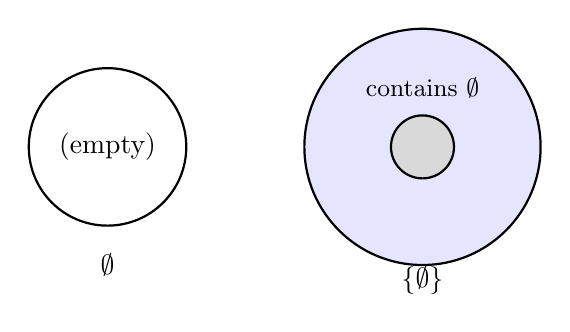
\begin{tikzpicture}
    % Empty set
    \draw[thick] (0,0) circle (1cm);
    \node at (0,-1.5) {$\emptyset$};
    \node at (0,0) {(empty)};
    
    % Set containing empty set
    \draw[thick, fill=blue!10] (4,0) circle (1.5cm);
    \draw[thick, fill=gray!30] (4,0) circle (0.4cm);
    \node at (4,-1.7) {$\{\emptyset\}$};
    \node[above] at (4,0.5) {\small contains $\emptyset$};
\end{tikzpicture}
\end{center}
\end{warning}

\subsection{Axiom 3: Pairing}

\begin{axiom}[Pairing]
\[\forall a \forall b \exists c \forall x (x \in c \iff x = a \lor x = b)\]
\end{axiom}

\begin{intuition}
\textbf{In words:} For any two sets $a$ and $b$, there exists a set $\{a, b\}$ containing exactly those two sets.

This lets us build finite sets!
\end{intuition}

\begin{example}
\begin{itemize}
    \item From $1$ and $2$, we get $\{1, 2\}$
    \item From $a$ and $a$, we get $\{a, a\} = \{a\}$ (singleton set)
    \item From $\emptyset$ and $\emptyset$, we get $\{\emptyset\}$
\end{itemize}
\end{example}

\begin{center}
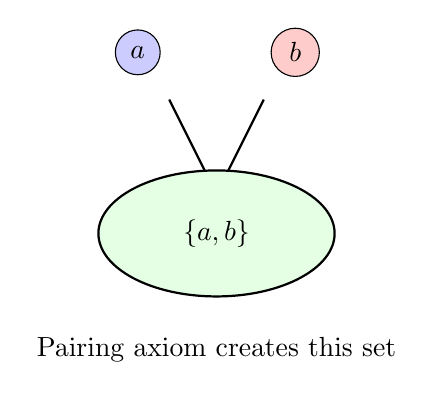
\begin{tikzpicture}
    \node[circle, draw, fill=blue!20] (a) at (0,0) {$a$};
    \node[circle, draw, fill=red!20] (b) at (2,0) {$b$};
    
    \draw[->, thick] (0.4,-0.6) -- (1,-1.8);
    \draw[->, thick] (1.6,-0.6) -- (1,-1.8);
    
    \draw[thick, fill=green!10] (1,-2.3) ellipse (1.5cm and 0.8cm);
    \node at (1,-2.3) {$\{a, b\}$};
    
    \node[below] at (1,-3.5) {Pairing axiom creates this set};
\end{tikzpicture}
\end{center}

\textbf{Building up:}
\begin{align*}
\{\emptyset\} &\text{ exists (from Pairing with } a = b = \emptyset \text{)} \\
\{\emptyset, \{\emptyset\}\} &\text{ exists (from Pairing)} \\
&\vdots
\end{align*}

\subsection{Axiom 4: Union}

\begin{axiom}[Union]
\[\forall \mathcal{F} \exists A \forall x (x \in A \iff \exists Y \in \mathcal{F} (x \in Y))\]
\end{axiom}

\begin{intuition}
\textbf{In words:} Given a collection of sets $\mathcal{F}$, there exists a set $A$ containing all elements that belong to at least one set in $\mathcal{F}$.

We write $A = \bigcup \mathcal{F}$ (``the union of $\mathcal{F}$'').
\end{intuition}

\begin{example}
Let $\mathcal{F} = \{\{1, 2\}, \{2, 3\}, \{3, 4\}\}$

Then $\bigcup \mathcal{F} = \{1, 2, 3, 4\}$ (all elements from all sets)
\end{example}

\begin{center}
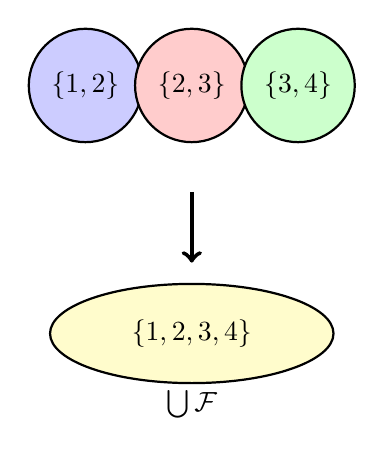
\begin{tikzpicture}[scale=0.9]
    % Three sets
    \draw[thick, fill=blue!20] (-1,0) circle (0.8cm);
    \node at (-1,0) {$\{1,2\}$};
    
    \draw[thick, fill=red!20] (0.5,0) circle (0.8cm);
    \node at (0.5,0) {$\{2,3\}$};
    
    \draw[thick, fill=green!20] (2,0) circle (0.8cm);
    \node at (2,0) {$\{3,4\}$};
    
    \draw[->, ultra thick] (0.5,-1.5) -- (0.5,-2.5);
    
    \draw[thick, fill=yellow!20] (0.5,-3.5) ellipse (2cm and 0.7cm);
    \node at (0.5,-3.5) {$\{1, 2, 3, 4\}$};
    
    \node at (0.5,-4.5) {$\bigcup \mathcal{F}$};
\end{tikzpicture}
\end{center}

\textbf{Binary union:} For sets $A$ and $B$:
\[A \cup B := \bigcup \{A, B\}\]

This is the usual ``union'' operation!

\subsection{Axiom 5: Power Set}

\begin{axiom}[Power Set]
\[\forall X \exists P \forall Y (Y \in P \iff Y \subseteq X)\]
\end{axiom}

\begin{intuition}
\textbf{In words:} For any set $X$, there exists a set $P$ containing all subsets of $X$.

We write $P = \mathcal{P}(X)$ or $P = 2^X$ (``the power set of $X$'').
\end{intuition}

First, what's a subset?

\begin{definition}[Subset]
\[A \subseteq B \iff \forall x (x \in A \implies x \in B)\]

``$A$ is a subset of $B$'' means every element of $A$ is also in $B$.
\end{definition}

\begin{example}
Let $X = \{1, 2\}$

Subsets of $X$: $\emptyset, \{1\}, \{2\}, \{1, 2\}$

Therefore: $\mathcal{P}(X) = \{\emptyset, \{1\}, \{2\}, \{1, 2\}\}$
\end{example}

\begin{center}
\begin{tikzpicture}[scale=0.8]
    % Original set
    \node[rectangle, draw, fill=blue!20, minimum width=2cm, minimum height=1cm] (X) at (0,2) {$X = \{1, 2\}$};
    
    % Power set container
    \node[rectangle, draw, fill=green!10, minimum width=6cm, minimum height=2.5cm] (P) at (0,-1.5) {};
    
    % Arrow connecting X to P
    \draw[->, ultra thick] (X.south) -- (P.north) node[midway, right=0.2cm] {\small take all subsets};
    
    \node at (0,-0.5) {$\mathcal{P}(X) =$};
    
    \node[draw, fill=red!20] at (-2.5,-1.5) {$\emptyset$};
    \node[draw, fill=red!20] at (-0.8,-1.5) {$\{1\}$};
    \node[draw, fill=red!20] at (0.8,-1.5) {$\{2\}$};
    \node[draw, fill=red!20] at (2.5,-1.5) {$\{1,2\}$};
    
    \node[below=0.3cm of P] {4 subsets $\implies |\mathcal{P}(X)| = 4 = 2^2$};
\end{tikzpicture}
\end{center}

\begin{theorem}[Cardinality of Power Set]
If $|X| = n$ (finite set with $n$ elements), then $|\mathcal{P}(X)| = 2^n$.
\end{theorem}

\begin{intuition}
For each element of $X$, you have a binary choice: include it in a subset or not.

$n$ elements $\times$ 2 choices each $= 2^n$ total subsets.
\end{intuition}

\subsection{Axiom 6: Separation (Specification)}

\begin{axiom}[Separation Schema]
For any formula $\phi(x)$ and set $A$:
\[\exists B \forall x (x \in B \iff x \in A \land \phi(x))\]
\end{axiom}

\begin{intuition}
\textbf{In words:} From any \textit{existing} set $A$, we can form the subset of elements satisfying a property $\phi$.

We write: $B = \{x \in A \mid \phi(x)\}$

\textbf{Warning on Notation:} In naive set theory, we often write $\{x \mid \phi(x)\}$. This is dangerous! It implies we are collecting objects from the entire universe. As Russell's Paradox showed, this leads to contradictions.

In axiomatic set theory, we must always specify \textbf{where} the elements come from: $\{x \in A \mid \dots\}$. We can only chip away from a block of marble (set $A$) that we already have; we cannot build a statue out of thin air.
\end{intuition}

\begin{keyidea}
This axiom \textbf{prevents Russell's Paradox}!

We can form $\{x \in A \mid x \notin x\}$ for any set $A$. This is well-defined and causes no contradiction.

But we \textbf{cannot} form $\{x \mid x \notin x\}$ (the problematic $R$ from Russell's Paradox). There's no universal set to filter from!
\end{keyidea}

\begin{example}
\begin{itemize}
    \item From $\mathbb{N}$, get $\{x \in \mathbb{N} \mid x \text{ is even}\} = \{0, 2, 4, 6, \ldots\}$
    \item From $\{1, 2, 3, 4, 5\}$, get $\{x \in \{1,2,3,4,5\} \mid x > 3\} = \{4, 5\}$
\end{itemize}
\end{example}

\subsection{Axiom 7: Infinity}

All axioms so far could be satisfied by finite sets only. We need infinity!

\begin{axiom}[Infinity]\index{axiom!of infinity}\index{infinity axiom}\index{ZFC axioms!infinity}\index{natural numbers!construction}
\[\exists I \left[\emptyset \in I \land \forall x (x \in I \implies x \cup \{x\} \in I)\right]\]
\end{axiom}

\begin{intuition}
\textbf{In words:} There exists a set $I$ containing:
\begin{itemize}
    \item The empty set $\emptyset$
    \item For every $x \in I$, also $x \cup \{x\}$ (the ``successor'' of $x$)
\end{itemize}

This set must be infinite!
\end{intuition}

\textbf{Building natural numbers:}
\begin{align*}
0 &:= \emptyset = \{\} \\
1 &:= 0 \cup \{0\} = \{\emptyset\} = \{0\} \\
2 &:= 1 \cup \{1\} = \{0\} \cup \{\{0\}\} = \{0, 1\} \\
3 &:= 2 \cup \{2\} = \{0, 1\} \cup \{\{0, 1\}\} = \{0, 1, 2\} \\
&\vdots \\
n &= \{0, 1, 2, \ldots, n-1\}
\end{align*}

This is the \textbf{von Neumann construction} of natural numbers!

\begin{center}
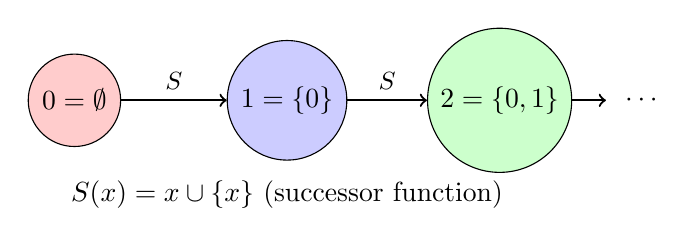
\begin{tikzpicture}[scale=0.9]
    \node[circle, draw, fill=red!20] (0) at (0,0) {$0 = \emptyset$};
    \node[circle, draw, fill=blue!20] (1) at (3,0) {$1 = \{0\}$};
    \node[circle, draw, fill=green!20] (2) at (6,0) {$2 = \{0,1\}$};
    \node at (8,0) {$\cdots$};
    
    \draw[->, thick] (0) -- (1) node[midway, above] {\small $S$};
    \draw[->, thick] (1) -- (2) node[midway, above] {\small $S$};
    \draw[->, thick] (2) -- (7.5,0);
    
    \node[below] at (3,-1) {$S(x) = x \cup \{x\}$ (successor function)};
\end{tikzpicture}
\end{center}

\begin{keyidea}
Every natural number is the \textit{set of all smaller natural numbers}!

$3 = \{0, 1, 2\}$ literally contains 0, 1, and 2 as elements.

This seems strange, but it works perfectly and lets us define arithmetic from pure set theory.
\end{keyidea}

\subsection{Axiom 8: Replacement}

\begin{remark}[On Functional Formulas]
The Replacement Axiom uses the notion of a ``functional relation'' or ``functional formula.'' Before we formally define functions as sets of ordered pairs (Chapter 6), we use this logical notion:

A formula $\phi(x, y)$ is \textbf{functional} if for each $x$, there exists a unique $y$ such that $\phi(x, y)$ holds:
\[\forall x \exists! y \, \phi(x, y)\]

This means: ``$\phi$ assigns to each $x$ exactly one $y$.''

\textbf{Examples:}
\begin{itemize}
    \item $\phi(x, y) := (y = x \cup \{x\})$ --- functional (successor operation)
    \item $\phi(x, y) := (y \in x)$ --- \textbf{not} functional (many $y$ can satisfy this)
\end{itemize}

This is \textit{not} circular: we're defining functions syntactically (as formulas in logic) here, and will later define them semantically (as sets of pairs) in Chapter 6.
\end{remark}

\begin{axiom}[Replacement Schema]\index{axiom!of replacement}\index{replacement axiom}\index{ZFC axioms!replacement}
If $\phi(x, y)$ is a functional formula, then the image of any set under $\phi$ is also a set.

Formally: For any formula $\phi(x, y)$ where $\forall x \exists! y \, \phi(x, y)$:
\[\forall A \exists B \forall y (y \in B \iff \exists x \in A \, \phi(x, y))\]
\end{axiom}

\begin{intuition}
\textbf{In words:} If you have a set $A$ and a function $F$, then $F[A] = \{F(x) : x \in A\}$ is also a set.

You can \textit{transform} each element of a set and collect the results.
\end{intuition}

\begin{example}
\begin{itemize}
    \item Let $A = \{1, 2, 3\}$ and $F(x) = x^2$
    \item Then $F[A] = \{1, 4, 9\}$ is a set (by Replacement)
\end{itemize}
\end{example}

\subsection{Axiom 9: Foundation (Regularity)}

\begin{axiom}[Foundation]
\[\forall x (x \neq \emptyset \implies \exists y \in x (y \cap x = \emptyset))\]
\end{axiom}

\begin{intuition}
\textbf{In words:} Every non-empty set contains an element disjoint from itself.

This prevents pathological situations like:
\begin{itemize}
    \item Sets containing themselves: $x \in x$
    \item Infinite descending chains: $\cdots \in x_2 \in x_1 \in x_0$
\end{itemize}
\end{intuition}

\begin{theorem}
No set contains itself: $\forall x (x \notin x)$.
\end{theorem}

\begin{proof}
Suppose $x \in x$. Consider the singleton $\{x\}$.

By Foundation, there exists $y \in \{x\}$ such that $y \cap \{x\} = \emptyset$.

Since $\{x\}$ has only one element, $y = x$.

So $x \cap \{x\} = \emptyset$.

But $x \in x$ (by assumption) and $x \in \{x\}$ (by definition of singleton).

Therefore $x \in x \cap \{x\}$, contradicting $x \cap \{x\} = \emptyset$. ✗

So $x \notin x$ for all $x$. ✓
\end{proof}

\begin{center}
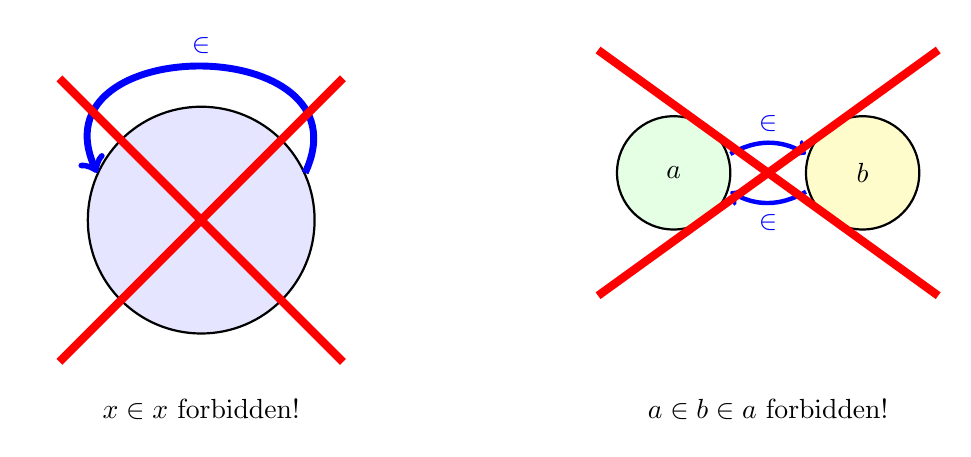
\begin{tikzpicture}[scale=1.2]
    % Left: Forbidden self-containment
    \draw[thick, fill=blue!10] (0,0) circle (1.2cm);
    \node at (0,0) {$x$};
    
    % Self-loop arrow - wider span on circle, moderate height
    \draw[->, line width=2.5pt, blue] (1.1,0.5) .. controls (1.8,2) and (-1.8,2) .. node[midway, above] {$\in$} (-1.1,0.5);
    
    % Big red X over the left diagram
    \draw[line width=3pt, red] (-1.5,-1.5) -- (1.5,1.5);
    \draw[line width=3pt, red] (-1.5,1.5) -- (1.5,-1.5);
    
    \node at (0,-2) {$x \in x$ forbidden!};
    
    % Right: Forbidden cycles
    \draw[thick, fill=green!10] (5,0.5) circle (0.6cm);
    \node at (5,0.5) {$a$};
    \draw[thick, fill=yellow!20] (7,0.5) circle (0.6cm);
    \node at (7,0.5) {$b$};
    
    % Arrows showing cycle
    \draw[->, ultra thick, blue] (5.6,0.7) to[bend left=30] node[midway, above] {$\in$} (6.4,0.7);
    \draw[->, ultra thick, blue] (6.4,0.3) to[bend left=30] node[midway, below] {$\in$} (5.6,0.3);
    
    % Big red X over the right diagram
    \draw[line width=3pt, red] (4.2,-0.8) -- (7.8,1.8);
    \draw[line width=3pt, red] (4.2,1.8) -- (7.8,-0.8);
    
    \node at (6,-2) {$a \in b \in a$ forbidden!};
\end{tikzpicture}
\end{center}

\subsection{Axiom 10: Choice}

\begin{axiom}[Axiom of Choice]\index{axiom!of choice}\index{choice, axiom of}\index{ZFC axioms!choice}
For any family of non-empty, pairwise disjoint sets, there exists a set containing exactly one element from each set in the family.
\end{axiom}

\begin{intuition}
\textbf{In words:} If you have a collection of boxes, each containing objects, you can simultaneously pick one object from each box.

Sounds obvious? It's surprisingly powerful (and controversial)!
\end{intuition}

\begin{example}
Suppose you have infinitely many pairs of shoes. You can choose the left shoe from each pair (definable rule).

But if you have infinitely many pairs of identical socks, how do you choose one from each pair? There's no rule! The Axiom of Choice says such a choice exists, even without a rule.
\end{example}

\begin{historicalnote}
The Axiom of Choice (AC) is \textbf{independent} of the other axioms. You can do mathematics with it (ZFC) or without it (ZF).

\textbf{Consequences of AC:}
\begin{itemize}
    \item ✓ Every vector space has a basis
    \item ✓ Tychonoff's theorem (topology)
    \item ✗ Banach-Tarski paradox (a ball can be split and reassembled into two identical balls!)
    \item ✗ Non-measurable sets exist
\end{itemize}

Most mathematicians accept AC because its positive consequences outweigh the weird ones. But some constructive mathematicians reject it.
\end{historicalnote}

\section{Building Mathematics from Sets}

Now that we have axioms, let's build!

\subsection{Defining Set Operations}

\textbf{Intersection:}
\[A \cap B := \{x \in A \mid x \in B\}\]

\begin{center}
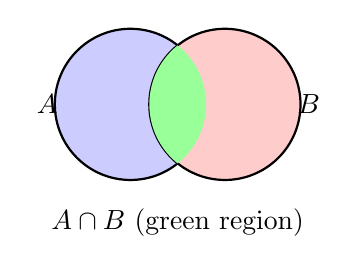
\begin{tikzpicture}[scale=0.8]
    \draw[thick, fill=blue!20] (0,0) circle (1.2cm);
    \draw[thick, fill=red!20] (1.5,0) circle (1.2cm);
    \begin{scope}
        \clip (0,0) circle (1.2cm);
        \fill[green!40] (1.5,0) circle (1.2cm);
    \end{scope}
    \node[left] at (-1,0) {$A$};
    \node[right] at (2.5,0) {$B$};
    \node[below] at (0.75,-1.5) {$A \cap B$ (green region)};
\end{tikzpicture}
\end{center}

\textbf{Difference:}
\[A \setminus B := \{x \in A \mid x \notin B\}\]

\textbf{Complement (relative to universe $U$):}
\[A^c := U \setminus A\]

\begin{warning}
There is NO universal set of all sets (this would lead to paradoxes). Complements are always relative to a fixed universe of discourse.
\end{warning}

\subsection{Ordered Pairs: A Clever Construction}

To define functions and relations, we need ordered pairs $(a, b)$ where order matters: $(a, b) \neq (b, a)$ unless $a = b$.

But we only have sets! How do we encode order?

\begin{definition}[Kuratowski Ordered Pair]
\[(a, b) := \{\{a\}, \{a, b\}\}\]
\end{definition}

\begin{intuition}
This definition is clever:
\begin{itemize}
    \item $\{a\}$ tells us what the first element is
    \item $\{a, b\}$ gives us both elements
    \item Together, we can recover $a$ and $b$ in order
\end{itemize}
\end{intuition}

\begin{theorem}[Characteristic Property]
\[(a, b) = (c, d) \iff a = c \land b = d\]
\end{theorem}

The proof is tedious but straightforward (consider cases).

\textbf{Key point:} Ordered pairs are just sets! Everything is sets.

\subsection{Cartesian Product}

\begin{definition}[Cartesian Product]
\[A \times B := \{(a, b) : a \in A, b \in B\}\]

More precisely: $A \times B := \{z : \exists a \in A \exists b \in B (z = (a, b))\}$
\end{definition}

\begin{example}
$\{1, 2\} \times \{a, b\} = \{(1,a), (1,b), (2,a), (2,b)\}$
\end{example}

\begin{center}
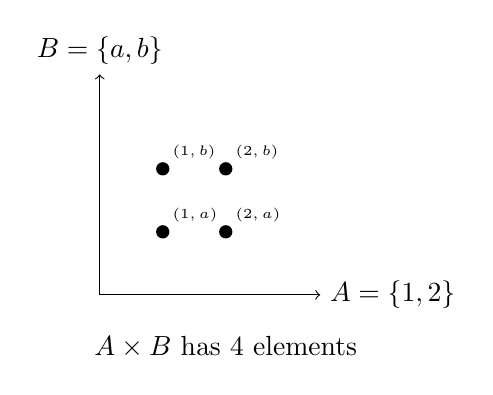
\begin{tikzpicture}[scale=0.8]
    % Grid
    \draw[->] (0,0) -- (3.5,0) node[right] {$A = \{1, 2\}$};
    \draw[->] (0,0) -- (0,3.5) node[above] {$B = \{a, b\}$};
    
    % Points
    \foreach \x/\xlabel in {1/1, 2/2} {
        \foreach \y/\ylabel in {1/a, 2/b} {
            \fill (\x,\y) circle (3pt);
            \node[above right] at (\x,\y) {\tiny $(\xlabel, \ylabel)$};
        }
    }
    
    \node[below] at (2,-0.5) {$A \times B$ has 4 elements};
\end{tikzpicture}
\end{center}

\section{Looking Forward}

We have built the universe of sets and defined the basic operations on them.

\begin{keyidea}
\textbf{What comes next?}

Sets are just the raw material. To do mathematics, we need to connect them.
\begin{itemize}
    \item \textbf{Chapter 4 (Relations)}: We will define how elements of sets relate to each other (e.g., ``less than'', ``equivalent to'').
    \item \textbf{Chapter 5 (Arithmetic)}: We will use equivalence relations to construct integers and rationals.
    \item \textbf{Chapter 6 (Functions)}: We will define special relations that map inputs to outputs.
    \item \textbf{Chapter 7 (Cardinality)}: We will use functions to measure the size of infinite sets.
\end{itemize}
\end{keyidea}

\vspace{1cm}
\noindent You now have the foundations. The mathematical universe is yours to explore.
